\documentclass[a4paper,titlepage,11pt,twosides,floatssmall]{mwrep}
\usepackage[left=2.5cm,right=2.5cm,top=2.5cm,bottom=2.5cm]{geometry}
\usepackage[OT1]{fontenc}
\usepackage{polski}
\usepackage{amsmath}
\usepackage{amsfonts}
\usepackage{amssymb}
\usepackage{graphicx}
\usepackage{float}
\usepackage{url}
\usepackage{tikz}
\usetikzlibrary{arrows,calc,decorations.markings,math,arrows.meta}
\usepackage{rotating}
\usepackage[percent]{overpic}
\usepackage[cp1250]{inputenc}
\usepackage{xcolor}
\usepackage{colortbl}
\usepackage{pgfplots}
\usetikzlibrary{pgfplots.groupplots}
\usepackage{listings}
\usepackage{matlab-prettifier}
\usepackage{enumitem,amssymb}
\definecolor{szary}{rgb}{0.95,0.95,0.95}
\usepackage{siunitx}
\usepackage{url}
\usepackage{caption}
\usepackage{refstyle}
\usepackage{multirow}
%\setlength{\textfloatsep}{5pt}
\raggedbottom
\sisetup{detect-weight,exponent-product=\cdot,output-decimal-marker={,},per-mode=symbol,binary-units=true,range-phrase={-},range-units=single}
\SendSettingsToPgf
%konfiguracje pakietu listings
\lstset{
	backgroundcolor=\color{szary},
	frame=single,
	breaklines=true,
}
\lstdefinestyle{customlatex}{
	basicstyle=\footnotesize\ttfamily,
	%basicstyle=\small\ttfamily,
}
\lstdefinestyle{customc}{
	breaklines=true,
	frame=tb,
	language=C,
	xleftmargin=0pt,
	showstringspaces=false,
	basicstyle=\small\ttfamily,
	keywordstyle=\bfseries\color{green!40!black},
	commentstyle=\itshape\color{purple!40!black},
	identifierstyle=\color{blue},
	stringstyle=\color{orange},
}
\lstdefinestyle{custommatlab}{
	captionpos=t,
	breaklines=true,
	frame=tb,
	xleftmargin=0pt,
	language=matlab,
	showstringspaces=false,
	basicstyle=\footnotesize\ttfamily,
	%basicstyle=\scriptsize\ttfamily,
	keywordstyle=\bfseries\color{green!40!black},
	commentstyle=\itshape\color{purple!40!black},
	identifierstyle=\color{blue},
	stringstyle=\color{orange},
}

%wymiar tekstu (bez �ywej paginy)
\textwidth 160mm \textheight 247mm

%ustawienia pakietu pgfplots
\pgfplotsset{
tick label style={font=\scriptsize},
label style={font=\small},
legend style={font=\small},
title style={font=\small}
}

\def\figurename{Rys.}
\def\tablename{Tab.}

%konfiguracja liczby p�ywaj�cych element�w
\setcounter{topnumber}{0}%2
\setcounter{bottomnumber}{3}%1
\setcounter{totalnumber}{5}%3
\renewcommand{\textfraction}{0.01}%0.2
\renewcommand{\topfraction}{0.95}%0.7
\renewcommand{\bottomfraction}{0.95}%0.3
\renewcommand{\floatpagefraction}{0.35}%0.5

\begin{document}
\frenchspacing
\pagestyle{uheadings}

%strona tytu�owa
\title{\bf Sprawozdanie z projektu i laboratorium nr 1 \\ Blok mobilny\vskip 0.1cm}
\author{Prowadz�cy: dr in�. Wojciech Dudek}
\author{Kaniuka Jan, Krasnod�bski Przemys�aw}
\date{2021}

\makeatletter
\renewcommand{\maketitle}{\begin{titlepage}
\begin{center}{\LARGE {\bf
Wydzia� Elektroniki i Technik Informacyjnych}}\\
\vspace{0.4cm}
{\LARGE {\bf Politechnika Warszawska}}\\
\vspace{0.3cm}
\end{center}
\vspace{5cm}
\begin{center}
{\bf \LARGE Sterowanie i symulacja robot�w\vskip 0.1cm}
\end{center}
\vspace{1cm}
\begin{center}
{\bf \LARGE \@title}
\end{center}
\vspace{2cm}
\begin{center}
{\bf \Large \@author \par}
\end{center}
\vspace*{\stretch{6}}
\begin{center}
\bf{\large{Warszawa, \@date\vskip 0.1cm}}
\end{center}
\end{titlepage}
}
\makeatother

\maketitle

\tableofcontents
\chapter{Wst�p}
Sprawozdanie zosta�o przygotowane w ramach zaj�� z przedmiotu \emph{Sterowanie i symulacja robot�w} w semestrze zimowym roku 2021. Cz�� laboratoryjna zosta�a zrealizowana podczas zaj�� w dniu 4.11.2021. Na laboratorium skupili�my si� na budowie �wiata i jego mapy. W cz�ci projektowej mieli�my za zadanie zaimplementowa� modu� planowania lokalnego. 


\begin{figure}[!htb]
    \centering
    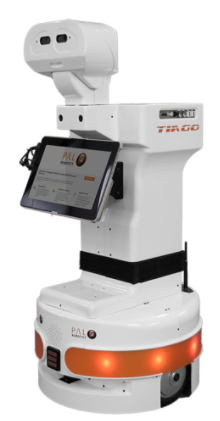
\includegraphics[scale=1]{plots/tiago}
    \caption{Robot \emph{Tiago} (\emph{Rico})}
		\label{fig:sampleFig}
\end{figure}
\chapter{Cz�� laboratoryjna}


\subsection{Budowa parterowego �wiata}  
Prac� na laboratorium zacz�li�my od budowy parterowego �wiata w symulatorze \texttt{Gazebo}. Zbudowali�my i zapisali�my dwa �wiaty: parterowy budynek oraz d�ugi korytarz bez drzwi. Model budynku b�dzie naszym �rodowiskiem testowym dla modu�u planowania implementowanego w czasie projektu. Drugi �wiat zostanie wykorzystany przy pracy z systemem lokalizacji \texttt{amcl} podczas laboratorium nr 3.

\subsection{Parterowy budynek z przej�ciami o r�nej szeroko�ci}  
Zbudowali�my budynek o prostym uk�adzie pomieszcze�. Umie�cili�my w nim przej�cia o r�nej szeroko�ci - odpowiednio 100\%, 150\%, 200\% i 300\% szeroko�ci robota. W cz�ci projektowej b�dziemy sprawdza�, jak warto�ci parametr�w map koszt�w oraz planer�w wp�ywaj� na zdolno�� robota do przejechania przed otw�r danej szeroko�ci.

\subsection{D�ugi korytarz bez drzwi}  
Utworzyli�my korytarz o jednolitych �cianach, bez drzwi oraz okien o d�ugo�ci 20 metr�w.

\subsection{Konfiguracja modu�u SLAM}  
Korzystali�my z modu�u \texttt{SLAM} (\textit{Simultaneous Localization and Mapping}) wykorzystuj�cego informacje z tematu \textit{/scan\_raw}. Pozwoli�o to na stworzenie dwuwymiarowej siatki zaj�to�ci.

\subsection{Budowa mapy}  
Zbudowanie mapy sprowadza�o si� do uruchomienia w�z�a pozwalaj�cego na sterowanie robotem za pomoc� klawiatury i na przejechaniu przez robota ca�ej powierzchni parterowego budynku.

\subsection{Pomiar �rednicy robota} 
Korzystaj�cz z narz�dzia \textit{Measure} w \texttt{RViZ} zmierzyli�my �rednic� bazy jezdnej robota, aby m�c j� p�niej uwzgl�dni� przy konfiguracji map koszt�w.

\begin{figure}[H]
    \centering
    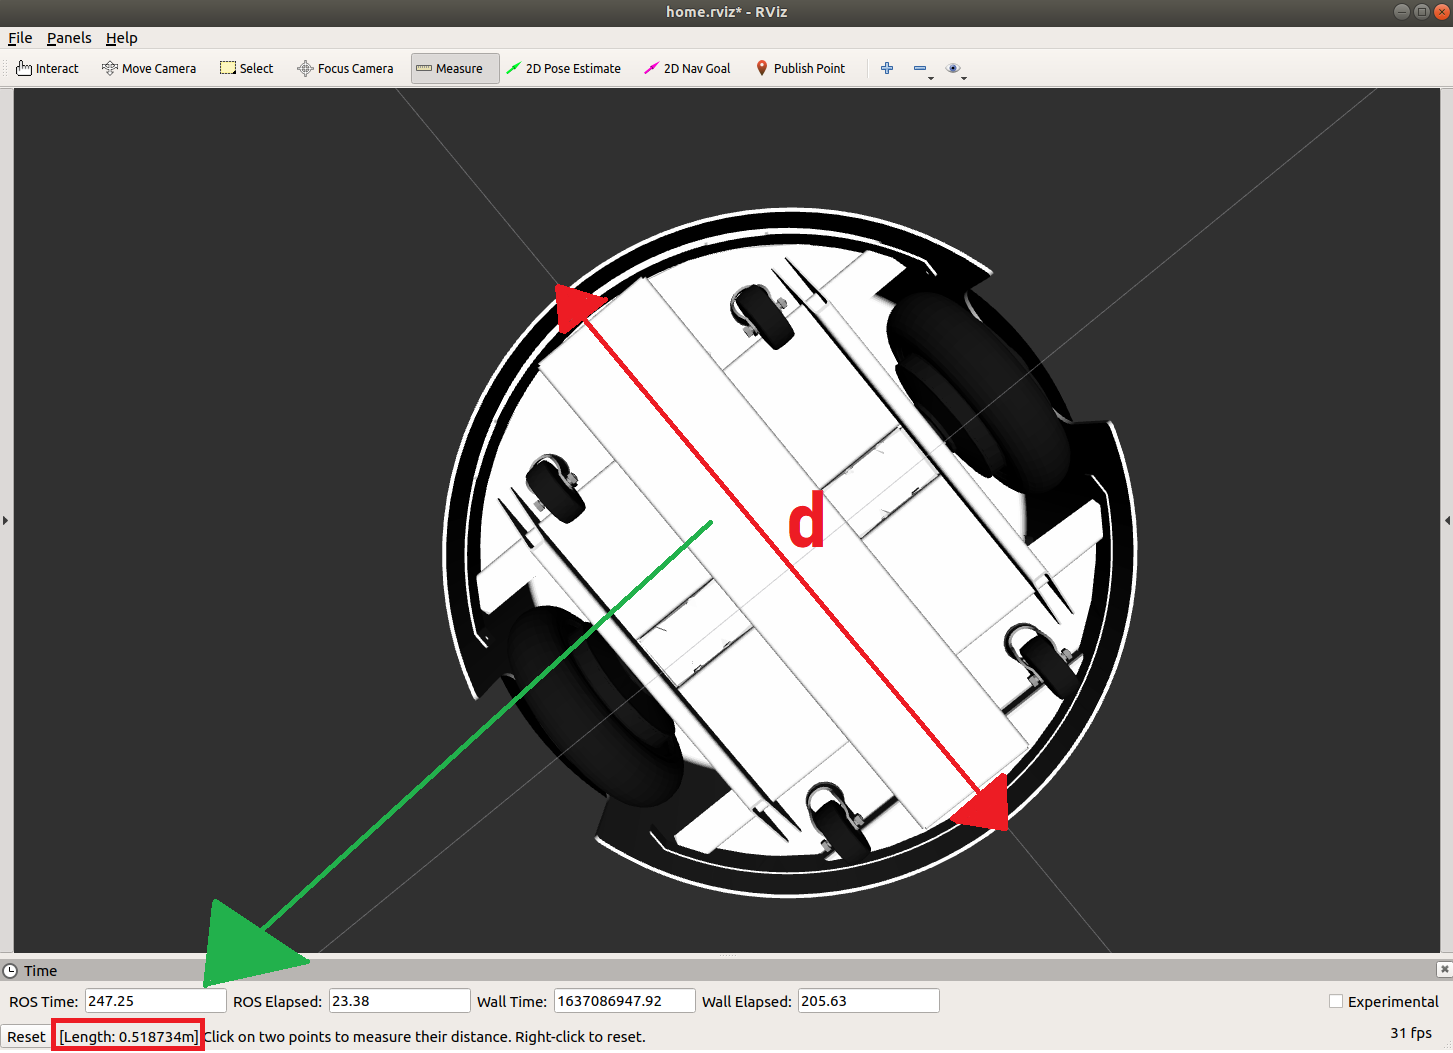
\includegraphics[scale=0.21]{Projekt_2/plots/diameter}
    \caption{Pomiar �rednicy bazy jezndej robota TiaGo.}
\end{figure}





\chapter{Cz�� projektowa}


\subsection{Implementacja wzgl�dnego sterowania pozycyjnego}  
Poni�ej zamieszczamy testy kwadratu dla trzech, r�nych warto�ci pr�dko�ci: liniowej i k�towej:

\begin{figure}[!htb]
    \centering
    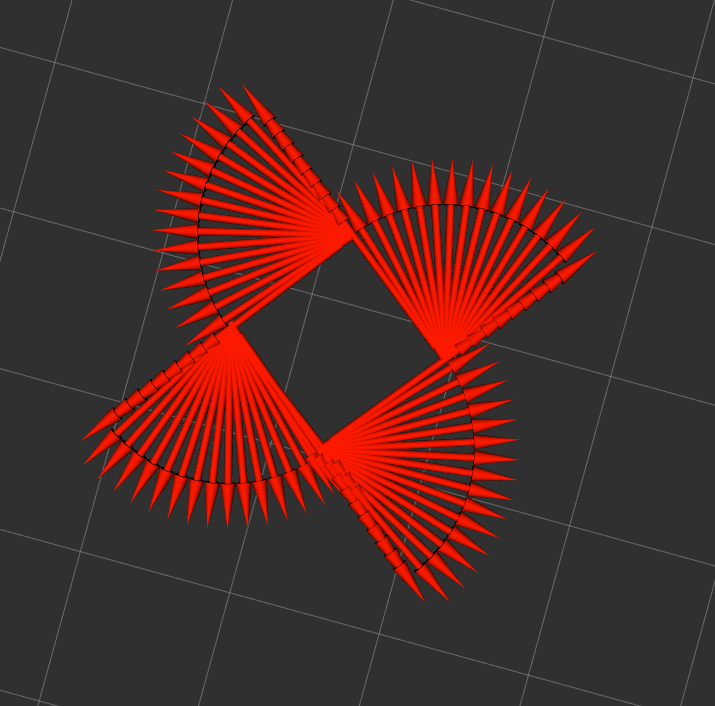
\includegraphics[scale=0.3]{Projekt_1/plots/square_vel_low}
    \caption{Pr�dko�� \emph{ma�a}}
\end{figure}

\begin{figure}[!htb]
    \centering
    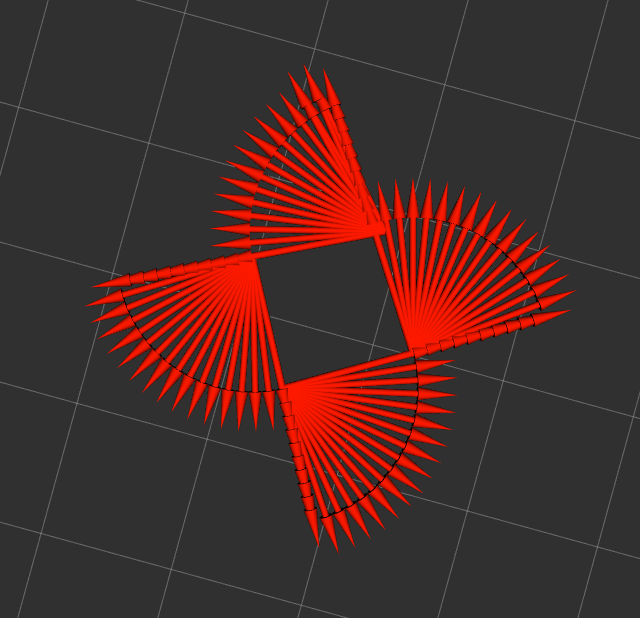
\includegraphics[scale=0.35]{Projekt_1/plots/square_vel_med}
    \caption{Pr�dko�� \emph{�rednia}}
\end{figure}

\begin{figure}[!htb]
    \centering
    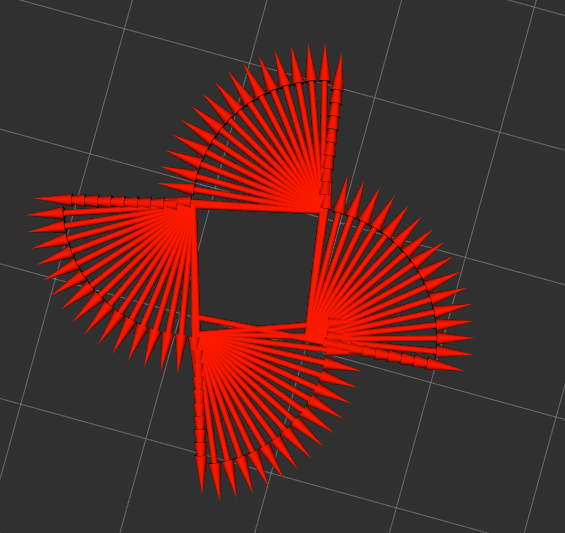
\includegraphics[scale=0.35]{Projekt_1/plots/square_vel_high}
    \caption{Pr�dko�� \emph{du�a}}
\end{figure}


\subsection{Por�wnanie dok�adno�ci osi�gania pozycji z wykorzystaniem pozycji referencyjnej}
Dokonali�my analizy dzia�ania wewn�trznych regulator�w robota podczas symulacji w reakcji na zadawane komendy ruchu. Przebiegi warto�ci zadanej i osi�ganych parametr�w ruchu przedstawiono na rysunkach poni�ej. Z powodu bardzo podobnych wynik�w dla r�nych pr�dko�ci i implementacji przedstawiono tylko niekt�re wykresy.
%\nopagebreak
\subsubsection{Sterowanie pr�dko�ciowe}
\nopagebreak
\begin{figure}[H]
    \centering
    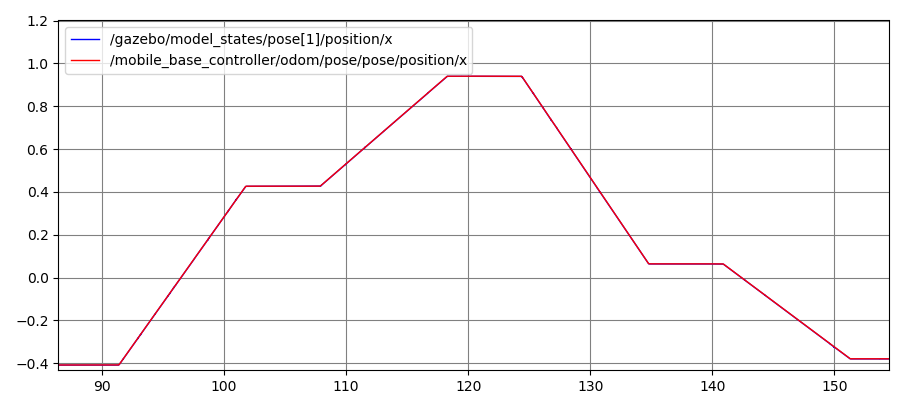
\includegraphics[scale=0.6]{Projekt_1/plots/time_medium}
		\caption{Pozycje liniowe x zadane i wykonane}
		
		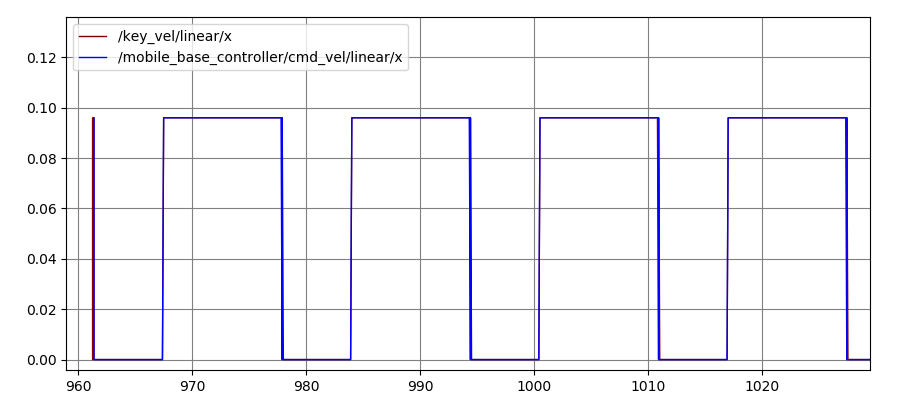
\includegraphics[scale=0.6]{Projekt_1/plots/time_medium_x}
		\caption{Pr�dko�ci liniowe x zadane i wykonane}
		
	  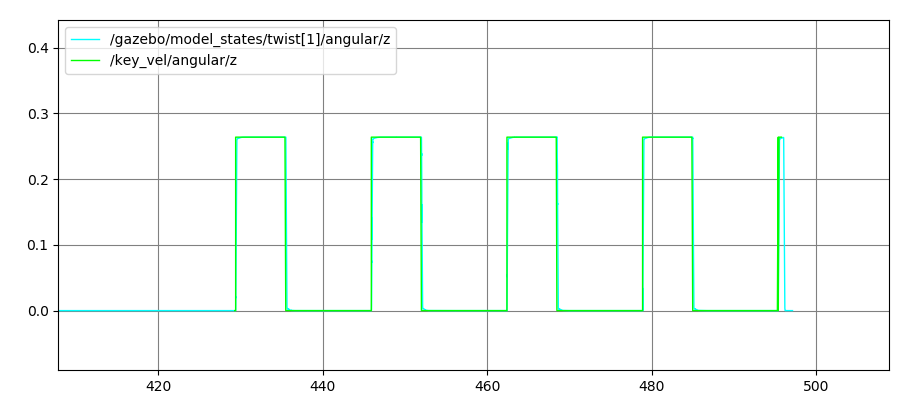
\includegraphics[scale=0.6]{Projekt_1/plots/time_medium_z}
		\caption{Pr�dko�ci k�towe zadane i wykonane}
\end{figure}



\subsubsection{Sterowanie z odometri�}

\begin{figure}[H]
    \centering
    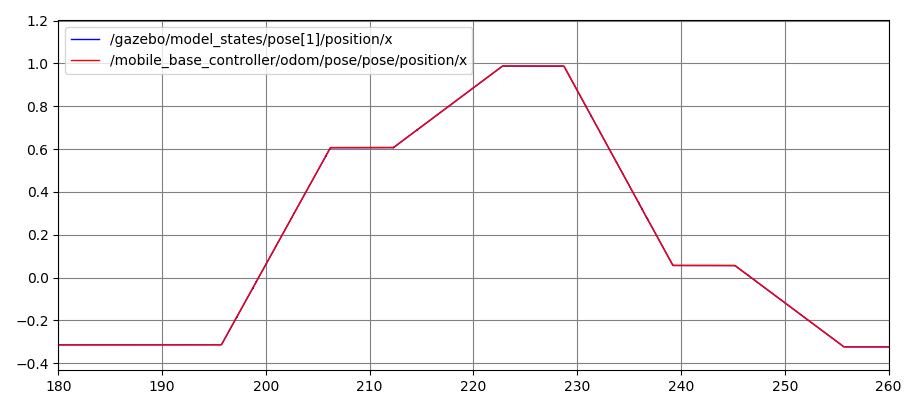
\includegraphics[scale=0.6]{Projekt_1/plots/odom_medium}
		\caption{Pozycje liniowe x zadane i wykonane}
		
		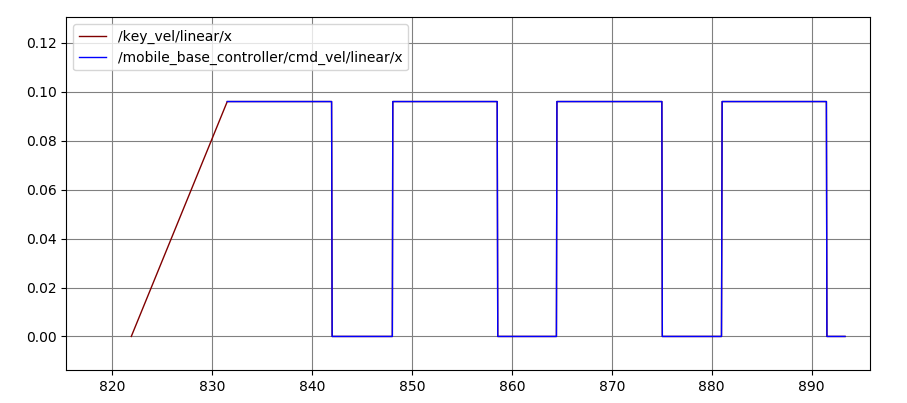
\includegraphics[scale=0.6]{Projekt_1/plots/odom_medium_x}
		\caption{Pr�dko�ci liniowe x zadane i wykonane}
		
		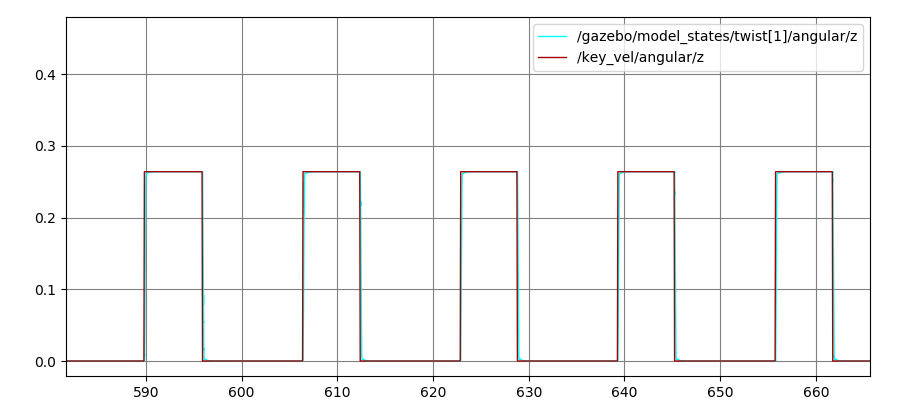
\includegraphics[scale=0.6]{Projekt_1/plots/odom_medium_z}
		\caption{Pr�dko�ci k�towe zadane i wykonane}
\end{figure}



Powy�sze dane zebrano podczas ruchu robota ze �redni� pr�dko�ci�. Wyra�nie wida�, �e pr�dko�ci oraz pozycje zadane s� r�wne referencyjnym. Ma�e rozbie�no�ci mo�na zauwa�y� podczas du�ych zmian warto�ci pr�dko�ci. Wynikaj� one ze sko�czonej warto�ci przy�pieszenia  robota.

\subsection{Praca z rzeczywistym robotem}  
Mieli�my mo�liwo�� uruchomienia naszych program�w na rzeczywistym robocie \emph{Tiago}. Celem zadania by�o zebranie danych do analizy por�wnawczej pomi�dzy lokalizacj� globaln�, a lokalizacj� wynikaj�c� z odometrii. Uruchomili�my program zadaj�cy ruch po kwadracie z wykorzystaniem odometrii dla trzech warto�ci pr�dko�ci.



\subsection{rosbag}
Podczas pracy z robotem zebrali�my dane, kt�re zosta�y poddane p�niejszej analizie. Przy u�yciu narz�dzia \emph{rosbag} mogli�my "nagra�" wiadomo�ci nadawane na wybranych tematach, aby m�c p�niej np. zwizualizowa� dane z pozycji na wykresie.\\
Zebrane dane pozyskali�my z temat�w: 
\begin{itemize}
	\item \texttt{/tf}
	\item \texttt{/mobile\_base\_controller/odom}
	\item \texttt{/robot\_pose}
\end{itemize} 

Poni�ej za��czyli�my dane obrazuj�ce przekszta�cenia pomi�dzy uk�adami \texttt{map} i \texttt{odom} w momencie startowym (na pocz�tku zbierania danych). R�nica w po�o�eniu tych uk�ad�w wsp�rz�dnych zostanie uwzgl�dniona podczas analizy danych opisanej w dalszej cz�ci sprawozdania.


\begin{figure}[!htb]
    \centering
    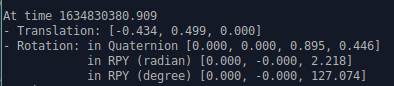
\includegraphics[scale=1]{Projekt_1/plots/conversion_low}
\end{figure}

\begin{figure}[!htb]
    \centering
    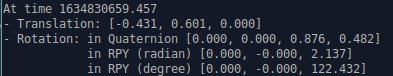
\includegraphics[scale=1]{Projekt_1/plots/conversion_med}
\end{figure}

\begin{figure}[!htb]
    \centering
    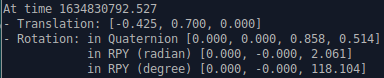
\includegraphics[scale=1.05]{Projekt_1/plots/conversion_high}
\end{figure}


\subsection{rqtplot}
Narz�dzie \texttt{rqt\_plot} pozwoli�o nam na wizualizacj� oraz por�wnywanie pr�dko�ci i/lub pozycji podczas przeprowadzania symulacji. Dzi�ki temu narz�dziu mogli�my zweryfikowa�, czy pr�dko�� zadana jest zgodna z pr�dko�ci� rzeczywist�.

Poni�szy wykres pokazuje, �e pr�dko�ci zadane oraz wykonane s� zgodne.
\begin{figure}[H]
    \centering
    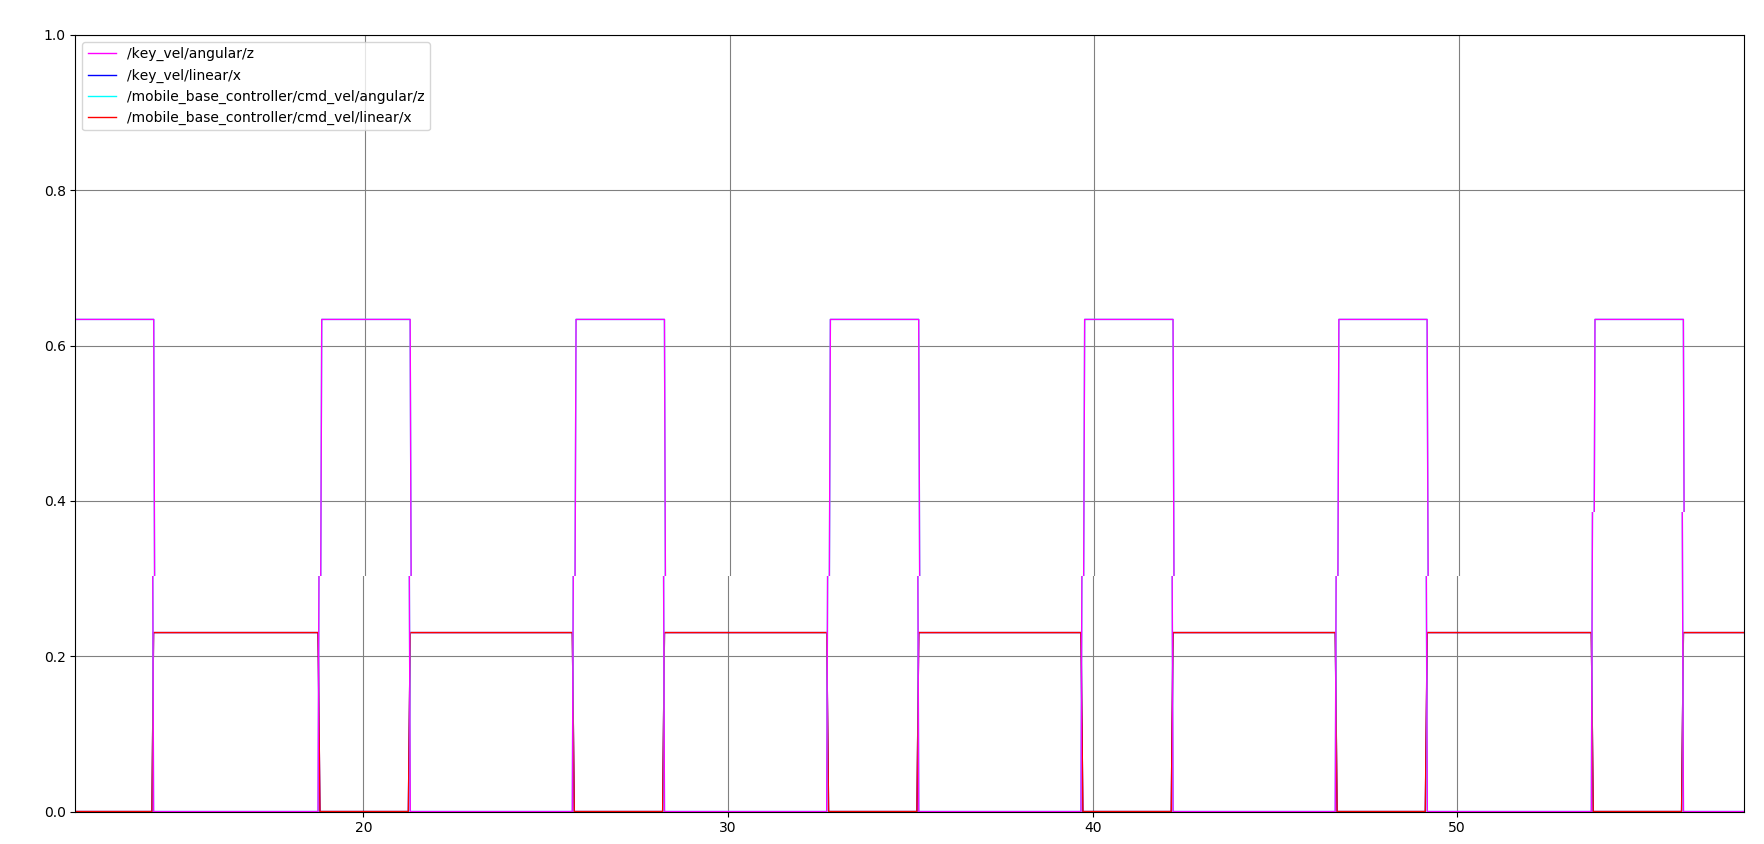
\includegraphics[scale=0.2]{Projekt_1/plots/velocities_odom}
		\caption{Pr�dko�ci zadane i wykonane}
\end{figure}

Narz�dzie \texttt{rqt\_plot} pozwoli�o nam r�wnie� na wizualizacj� danych obrazujacych pozycj� referencyjn� robota.

\begin{figure}[H]
    \centering
    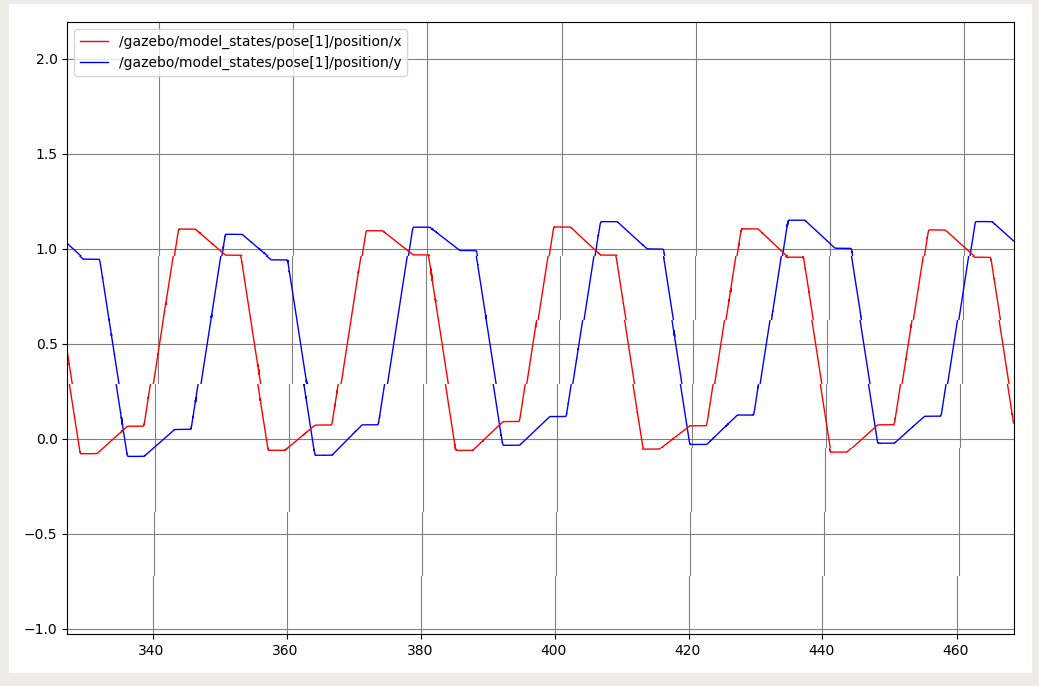
\includegraphics[scale=0.3]{Projekt_1/plots/talker_odometria}
		\caption{Pozycja robota z \emph{Gazebo}}
\end{figure}





\subsection{Analiza danych z pliku \emph{.bag} }
Dane odometryczne w temacie \texttt{/mobile\_base\_controller/odom} s� wyra�one w uk�adzie \texttt{odom}, a dane z lokalizacji globalnej w uk�adzie \texttt{map}. Transformacja mi�dzy tymi uk�adami jest zmienna w trakcie pracy robota i wynika z dzia�ania algorytmu globalnej lokalizacji. Zatem, aby por�wna� lokalizacj� robota na podstawie odometrii oraz lokalizacj� z fuzj� innych danych sensorycznych nale�y por�wnywa� dane z obu wskazanych temat�w wzgl�dem wsp�lnego uk�adu wsp�rz�dnych. Za ten uk�ad nale�y przyj�� uk�ad \texttt{map}. \\
Przekszta�cenie wykonali�my zgodnie z poni�sz� grafik� ( slajd z wyk�adu \emph{Wst�p do robotyki} autorstwa dr hab. in�. Wojciecha Szynkiewicza, EiTI PW) 

\begin{figure}[H]
    \centering
    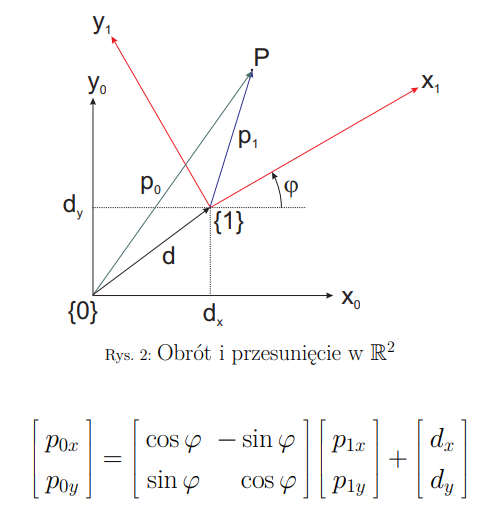
\includegraphics[scale=0.85]{Projekt_1/plots/wr_przekszt}
		\caption{Transformacja mi�dzy uk�adami wsp�rz�dnych na p�aszczy�nie}
\end{figure}

\subsubsection{Ruch rzeczywistego robota}
\begin{figure}[H]
    \centering
		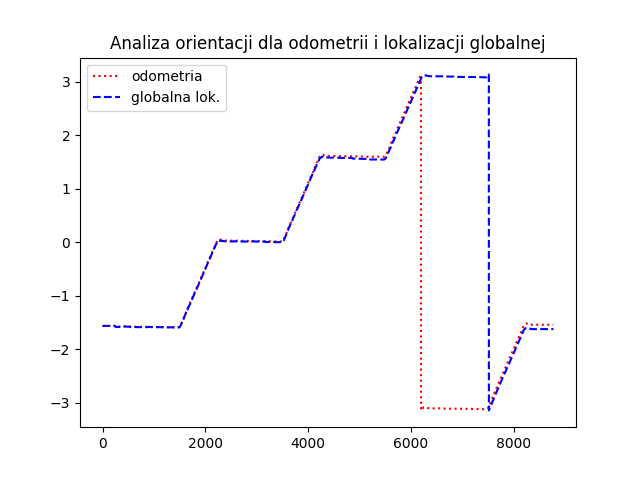
\includegraphics[scale=0.7]{Projekt_1/plots/low_comparison_2}
    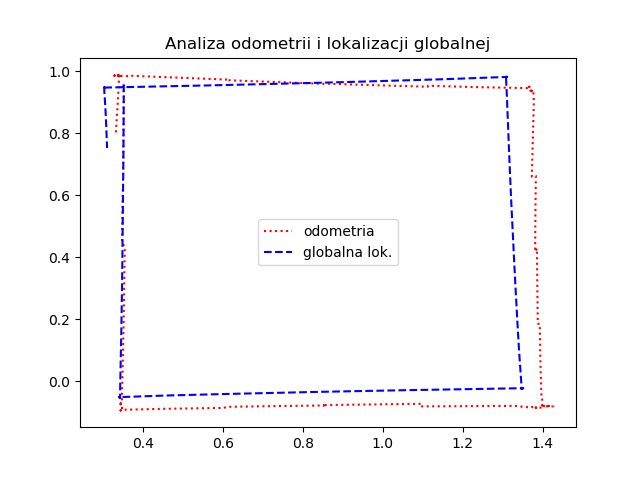
\includegraphics[scale=0.7]{plots/low_comparison}
		\caption{Test kwadratu z odometri�, pr�dko�� niska}
\end{figure}

\begin{figure}[H]
    \centering
		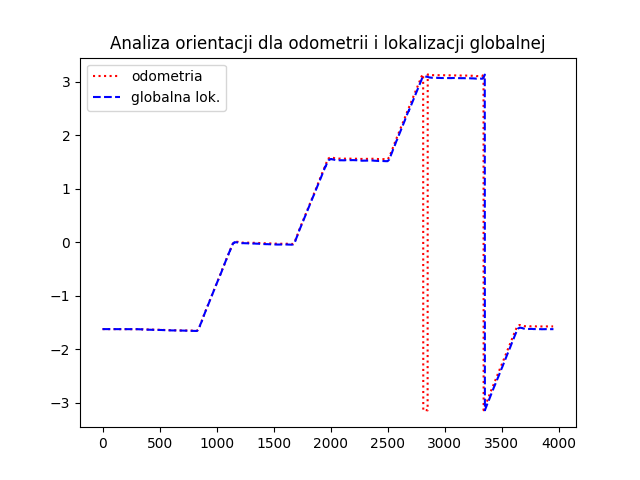
\includegraphics[scale=0.7]{Projekt_1/plots/med_comparison_2}
    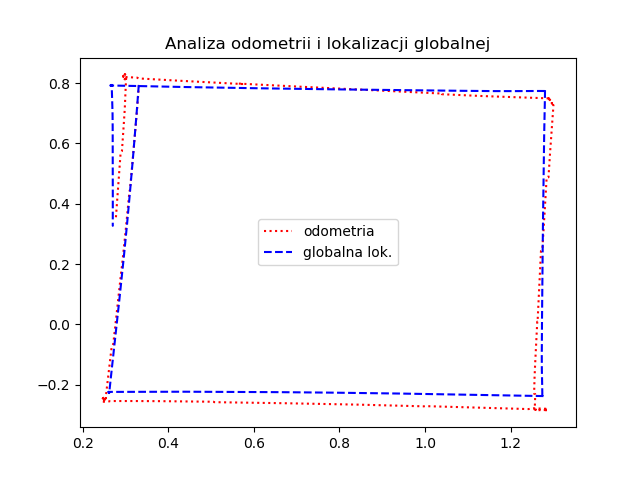
\includegraphics[scale=0.7]{plots/med_comparison}
		\caption{Test kwadratu z odometri�, pr�dko�� �rednia}
\end{figure}

\begin{figure}[H]
    \centering
		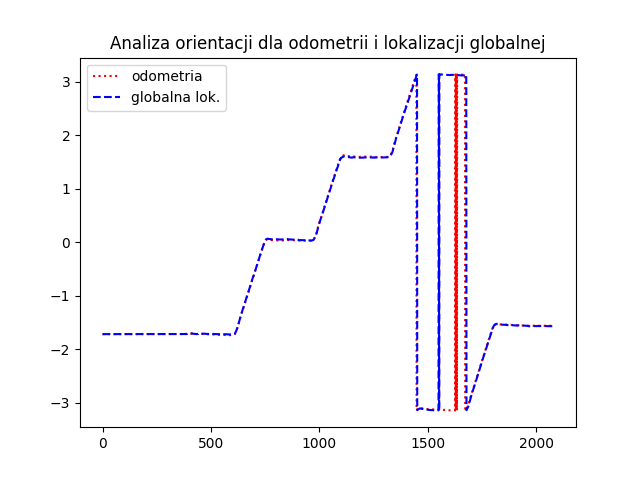
\includegraphics[scale=0.7]{Projekt_1/plots/high_comparison_2}
    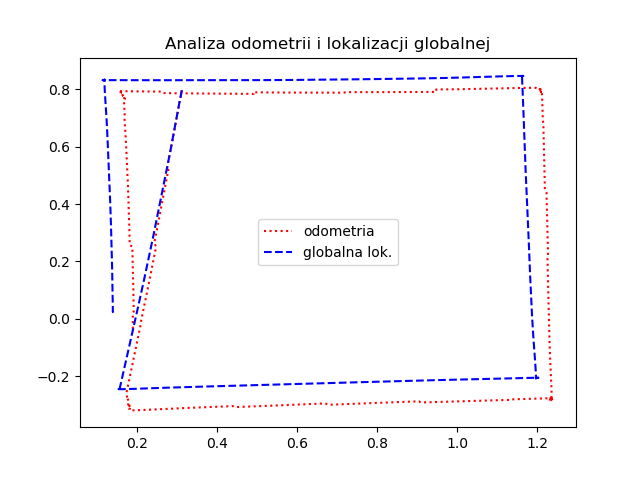
\includegraphics[scale=0.7]{plots/high_comparison}
		\caption{Test kwadratu z odometri�, pr�dko�� wysoka}
\end{figure}

Przedstawione przebiegi orientacji dla odometrii i lokalizacji globalnej s� ze sob� zgodne. Widoczne rozbie�no�ci wynikaj� z niewielkich b��d�w/szum�w pomiarowych i faktu zawierania si� miary k�towej w zakresie od -$\pi$ do $\pi$.


\subsubsection{Wyniki pomiar�w}

\begin{table}[H]
\caption{Por�wnanie b��d�w pozycji dla r�nych pr�dko�ci}
\label{t_wyrownanie_do_znaku_przecinek2}
\centering
\begin{tabular}{|c|c|c|c|c|c|c|}
\hline
\multirow{2}{*}{Pr�dko��} & \multicolumn{2}{c|}{B��d x} & \multicolumn{2}{c|}{B��d y} & \multicolumn{2}{c|}{B��d theta} \\ \cline{2-7} 
                          & Skumulowany     & �redni    & Skumulowany     & �redni    & Skumulowany       & �redni      \\ \hline
low                       & 61.17           & 0.0294    & 92.95           & 0.0447    & 521               & 0.2506      \\ \hline
medium                    & 48.06           & 0.0122    & 99.35           & 0.0252    & 6327              & 1.6018      \\ \hline
high                      & 276.52          & 0.0315    & 308.98          & 0.0352    & 19730             & 2.2498      \\ \hline
\end{tabular}
\end{table}

W przypadku zbyt szybkich ruch�w robota tracimy dok�adno�c pozycjonowania go w przestrzeni. Ograniczone przy�pieszenie robota wp�ywa szczeg�lnie na niedok�adno�c ruchu obrotowego, przez co dok�adne wykonanie wyznaczonej trajektori mo�e by� awykonalne.


\subsection{Struktura komunikacji}
W celu zobrazowania struktury steruj�cej robotem \emph{Tiago} w ramach ROS ( \emph{Robot Operating System}) za��czmy poni�ej grafy struktur komunikacji tzn. zale�no�ci pomi�dzy poszczeg�lnymi w�z�ami i tematami.

\begin{figure}[!htb]
    \centering
    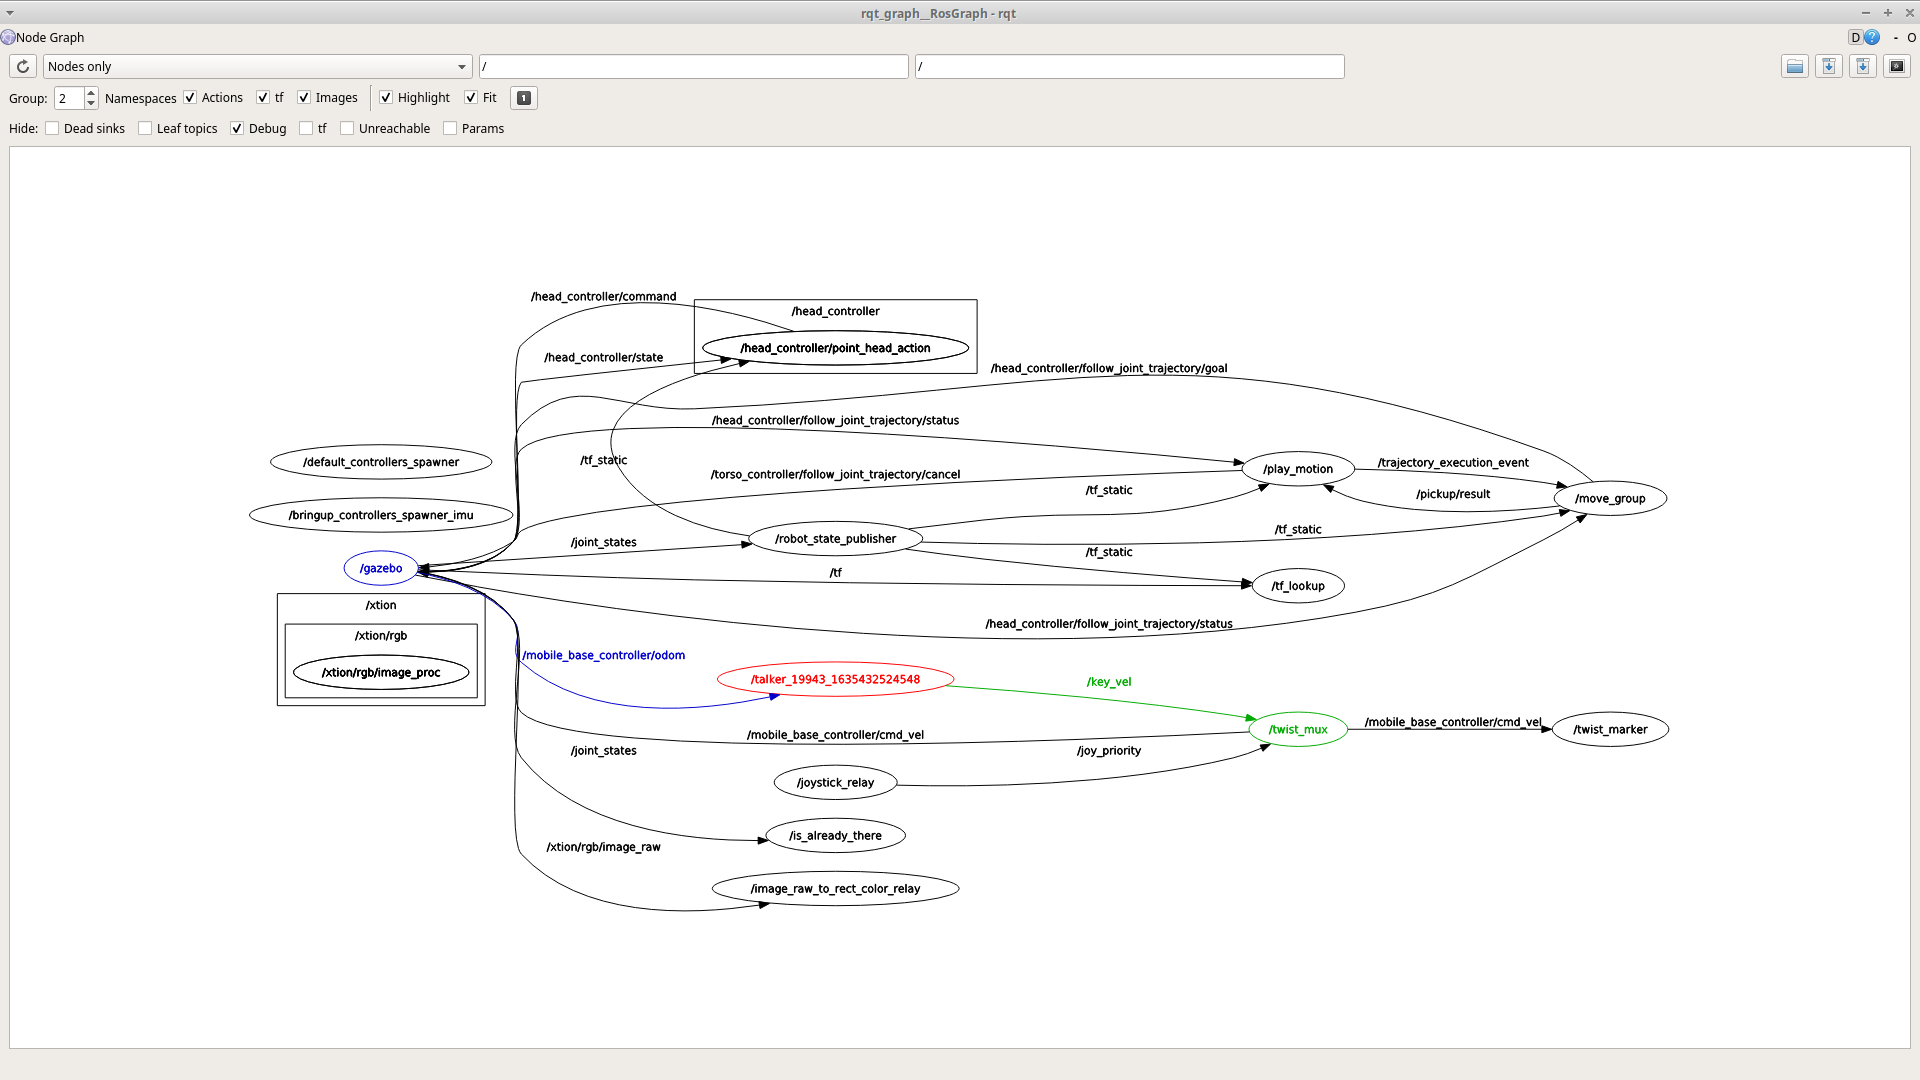
\includegraphics[scale=0.2]{Projekt_1/plots/graph_odometria2}
		\caption{Sterowanie z odometri� - struktura komunikacji}
\end{figure}

\begin{figure}[!htb]
    \centering
    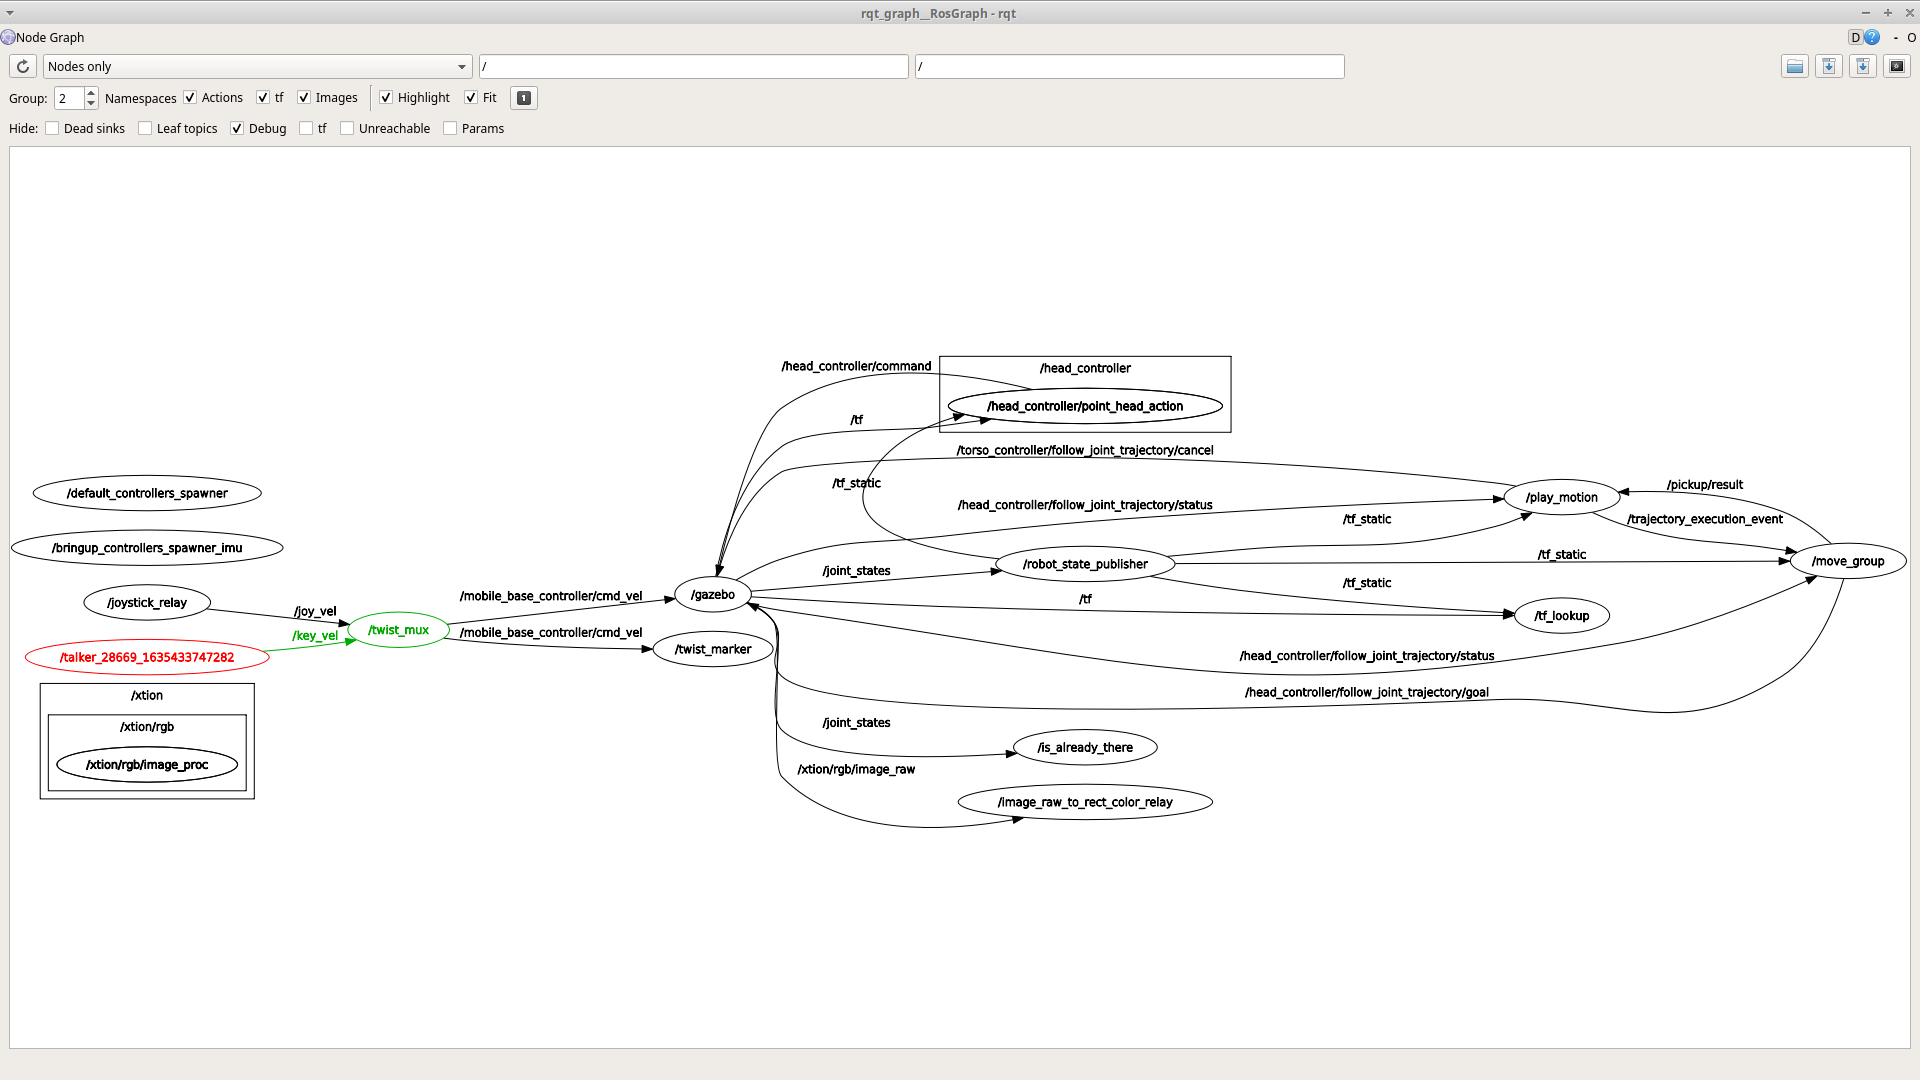
\includegraphics[scale=0.2]{Projekt_1/plots/graph_predkoscowe2}
		\caption{Sterowanie wy��cznie pr�dko�ciowe - struktura komunikacji}
\end{figure}






\chapter{Podsumowanie}

\subsection{Obserwacje i wnioski}  
Zaimplementowany modu� planowania zosta� poddany licznym testom w �rodowisku symulacyjnym. Pocz�tkowo wyznaczanie �cie�ki przez planer globalny nie dzia�a�o idelanie - wynika�o to z konfiguracji parametr�w w plikach \textit{.yaml}. Mnogo�� tych�e parametr�w by�a podstawow� trudno�ci� podczas wst�pnych konfiguracji. Z czasem jednak uda�o nam si� dobra� parametry, przy kt�rych planowanie �cie�ki oraz jej wykonanie przez robota mo�na by�o oceni� jako "zadowalaj�ce". Przy finalnie ustalonych warto�ciach parametr�w robot by� wstanie przejecha� przez przej�cie o ka�dej z szeroko�ci zaimplementowanych podczas laboratorium.
\bigbreak
Na etapie test�w badali�my r�wnie� dzia�anie planera lokalnego w reakcji na rekonfiguracj� �rodowiska. Podczas wykonywania �cie�ki przez robota dodawali�my na trasie przeszkody w postaci bry� (kula, sze�cian). Robot omija� przeszkod� wyznaczaj�c tras� przy wykorzystaniu modu�u planowania lokalnego.
\end{document}

